% Options for packages loaded elsewhere
\PassOptionsToPackage{unicode}{hyperref}
\PassOptionsToPackage{hyphens}{url}
%
\documentclass[
]{article}
\usepackage{amsmath,amssymb}
\usepackage{iftex}
\ifPDFTeX
  \usepackage[T1]{fontenc}
  \usepackage[utf8]{inputenc}
  \usepackage{textcomp} % provide euro and other symbols
\else % if luatex or xetex
  \usepackage{unicode-math} % this also loads fontspec
  \defaultfontfeatures{Scale=MatchLowercase}
  \defaultfontfeatures[\rmfamily]{Ligatures=TeX,Scale=1}
\fi
\usepackage{lmodern}
\ifPDFTeX\else
  % xetex/luatex font selection
\fi
% Use upquote if available, for straight quotes in verbatim environments
\IfFileExists{upquote.sty}{\usepackage{upquote}}{}
\IfFileExists{microtype.sty}{% use microtype if available
  \usepackage[]{microtype}
  \UseMicrotypeSet[protrusion]{basicmath} % disable protrusion for tt fonts
}{}
\makeatletter
\@ifundefined{KOMAClassName}{% if non-KOMA class
  \IfFileExists{parskip.sty}{%
    \usepackage{parskip}
  }{% else
    \setlength{\parindent}{0pt}
    \setlength{\parskip}{6pt plus 2pt minus 1pt}}
}{% if KOMA class
  \KOMAoptions{parskip=half}}
\makeatother
\usepackage{xcolor}
\usepackage[margin=1in]{geometry}
\usepackage{color}
\usepackage{fancyvrb}
\newcommand{\VerbBar}{|}
\newcommand{\VERB}{\Verb[commandchars=\\\{\}]}
\DefineVerbatimEnvironment{Highlighting}{Verbatim}{commandchars=\\\{\}}
% Add ',fontsize=\small' for more characters per line
\usepackage{framed}
\definecolor{shadecolor}{RGB}{248,248,248}
\newenvironment{Shaded}{\begin{snugshade}}{\end{snugshade}}
\newcommand{\AlertTok}[1]{\textcolor[rgb]{0.94,0.16,0.16}{#1}}
\newcommand{\AnnotationTok}[1]{\textcolor[rgb]{0.56,0.35,0.01}{\textbf{\textit{#1}}}}
\newcommand{\AttributeTok}[1]{\textcolor[rgb]{0.13,0.29,0.53}{#1}}
\newcommand{\BaseNTok}[1]{\textcolor[rgb]{0.00,0.00,0.81}{#1}}
\newcommand{\BuiltInTok}[1]{#1}
\newcommand{\CharTok}[1]{\textcolor[rgb]{0.31,0.60,0.02}{#1}}
\newcommand{\CommentTok}[1]{\textcolor[rgb]{0.56,0.35,0.01}{\textit{#1}}}
\newcommand{\CommentVarTok}[1]{\textcolor[rgb]{0.56,0.35,0.01}{\textbf{\textit{#1}}}}
\newcommand{\ConstantTok}[1]{\textcolor[rgb]{0.56,0.35,0.01}{#1}}
\newcommand{\ControlFlowTok}[1]{\textcolor[rgb]{0.13,0.29,0.53}{\textbf{#1}}}
\newcommand{\DataTypeTok}[1]{\textcolor[rgb]{0.13,0.29,0.53}{#1}}
\newcommand{\DecValTok}[1]{\textcolor[rgb]{0.00,0.00,0.81}{#1}}
\newcommand{\DocumentationTok}[1]{\textcolor[rgb]{0.56,0.35,0.01}{\textbf{\textit{#1}}}}
\newcommand{\ErrorTok}[1]{\textcolor[rgb]{0.64,0.00,0.00}{\textbf{#1}}}
\newcommand{\ExtensionTok}[1]{#1}
\newcommand{\FloatTok}[1]{\textcolor[rgb]{0.00,0.00,0.81}{#1}}
\newcommand{\FunctionTok}[1]{\textcolor[rgb]{0.13,0.29,0.53}{\textbf{#1}}}
\newcommand{\ImportTok}[1]{#1}
\newcommand{\InformationTok}[1]{\textcolor[rgb]{0.56,0.35,0.01}{\textbf{\textit{#1}}}}
\newcommand{\KeywordTok}[1]{\textcolor[rgb]{0.13,0.29,0.53}{\textbf{#1}}}
\newcommand{\NormalTok}[1]{#1}
\newcommand{\OperatorTok}[1]{\textcolor[rgb]{0.81,0.36,0.00}{\textbf{#1}}}
\newcommand{\OtherTok}[1]{\textcolor[rgb]{0.56,0.35,0.01}{#1}}
\newcommand{\PreprocessorTok}[1]{\textcolor[rgb]{0.56,0.35,0.01}{\textit{#1}}}
\newcommand{\RegionMarkerTok}[1]{#1}
\newcommand{\SpecialCharTok}[1]{\textcolor[rgb]{0.81,0.36,0.00}{\textbf{#1}}}
\newcommand{\SpecialStringTok}[1]{\textcolor[rgb]{0.31,0.60,0.02}{#1}}
\newcommand{\StringTok}[1]{\textcolor[rgb]{0.31,0.60,0.02}{#1}}
\newcommand{\VariableTok}[1]{\textcolor[rgb]{0.00,0.00,0.00}{#1}}
\newcommand{\VerbatimStringTok}[1]{\textcolor[rgb]{0.31,0.60,0.02}{#1}}
\newcommand{\WarningTok}[1]{\textcolor[rgb]{0.56,0.35,0.01}{\textbf{\textit{#1}}}}
\usepackage{longtable,booktabs,array}
\usepackage{calc} % for calculating minipage widths
% Correct order of tables after \paragraph or \subparagraph
\usepackage{etoolbox}
\makeatletter
\patchcmd\longtable{\par}{\if@noskipsec\mbox{}\fi\par}{}{}
\makeatother
% Allow footnotes in longtable head/foot
\IfFileExists{footnotehyper.sty}{\usepackage{footnotehyper}}{\usepackage{footnote}}
\makesavenoteenv{longtable}
\usepackage{graphicx}
\makeatletter
\def\maxwidth{\ifdim\Gin@nat@width>\linewidth\linewidth\else\Gin@nat@width\fi}
\def\maxheight{\ifdim\Gin@nat@height>\textheight\textheight\else\Gin@nat@height\fi}
\makeatother
% Scale images if necessary, so that they will not overflow the page
% margins by default, and it is still possible to overwrite the defaults
% using explicit options in \includegraphics[width, height, ...]{}
\setkeys{Gin}{width=\maxwidth,height=\maxheight,keepaspectratio}
% Set default figure placement to htbp
\makeatletter
\def\fps@figure{htbp}
\makeatother
\setlength{\emergencystretch}{3em} % prevent overfull lines
\providecommand{\tightlist}{%
  \setlength{\itemsep}{0pt}\setlength{\parskip}{0pt}}
\setcounter{secnumdepth}{-\maxdimen} % remove section numbering
\ifLuaTeX
  \usepackage{selnolig}  % disable illegal ligatures
\fi
\IfFileExists{bookmark.sty}{\usepackage{bookmark}}{\usepackage{hyperref}}
\IfFileExists{xurl.sty}{\usepackage{xurl}}{} % add URL line breaks if available
\urlstyle{same}
\hypersetup{
  pdftitle={Time Series Construction Labor in Tucurui and Altamira},
  hidelinks,
  pdfcreator={LaTeX via pandoc}}

\title{Time Series Construction Labor in Tucurui and Altamira}
\author{}
\date{\vspace{-2.5em}}

\begin{document}
\maketitle

In this R notebook, I will conduct a Time Series Analysis of Labor
Turnover in the cities of Tucuruí and Altamira, situated in the state of
Pará, Brazil.

\begin{Shaded}
\begin{Highlighting}[]
\FunctionTok{list.files}\NormalTok{(}\AttributeTok{path =} \StringTok{"../input"}\NormalTok{)}
\end{Highlighting}
\end{Shaded}

\begin{verbatim}
## character(0)
\end{verbatim}

\hypertarget{loading-libraries}{%
\subsection{Loading Libraries}\label{loading-libraries}}

\begin{Shaded}
\begin{Highlighting}[]
\FunctionTok{library}\NormalTok{(readr)}
\FunctionTok{library}\NormalTok{(tidyverse)}
\end{Highlighting}
\end{Shaded}

\begin{verbatim}
## -- Attaching core tidyverse packages ------------------------ tidyverse 2.0.0 --
## v dplyr     1.1.4     v purrr     1.0.2
## v forcats   1.0.0     v stringr   1.5.1
## v ggplot2   3.4.4     v tibble    3.2.1
## v lubridate 1.9.3     v tidyr     1.3.0
## -- Conflicts ------------------------------------------ tidyverse_conflicts() --
## x dplyr::filter() masks stats::filter()
## x dplyr::lag()    masks stats::lag()
## i Use the conflicted package (<http://conflicted.r-lib.org/>) to force all conflicts to become errors
\end{verbatim}

\begin{Shaded}
\begin{Highlighting}[]
\FunctionTok{library}\NormalTok{(lubridate)}
\FunctionTok{library}\NormalTok{(ggplot2)}
\FunctionTok{library}\NormalTok{(forecast)}
\end{Highlighting}
\end{Shaded}

\begin{verbatim}
## Registered S3 method overwritten by 'quantmod':
##   method            from
##   as.zoo.data.frame zoo
\end{verbatim}

\begin{Shaded}
\begin{Highlighting}[]
\FunctionTok{library}\NormalTok{(tseries)}
\FunctionTok{library}\NormalTok{(purrr)}
\FunctionTok{library}\NormalTok{(reshape2)}
\end{Highlighting}
\end{Shaded}

\begin{verbatim}
## 
## Attaching package: 'reshape2'
## 
## The following object is masked from 'package:tidyr':
## 
##     smiths
\end{verbatim}

\hypertarget{read}{%
\subsection{Read}\label{read}}

\begin{Shaded}
\begin{Highlighting}[]
\NormalTok{df }\OtherTok{\textless{}{-}} \FunctionTok{read\_csv}\NormalTok{(}\StringTok{"rais\_altamira\_tucurui\_updated.csv"}\NormalTok{)}
\end{Highlighting}
\end{Shaded}

\begin{verbatim}
## Rows: 191 Columns: 55
## -- Column specification --------------------------------------------------------
## Delimiter: ","
## dbl  (54): PopAltamira, PopTucurui, ShutAltamira, ShutTucurui, AdmAltamira, ...
## date  (1): Time
## 
## i Use `spec()` to retrieve the full column specification for this data.
## i Specify the column types or set `show_col_types = FALSE` to quiet this message.
\end{verbatim}

\hypertarget{check-the-structure-of-the-dataframe-look-for-missing-values-and-check-duplicate-rows}{%
\subsection{Check the structure of the dataframe, look for missing
values, and check duplicate
rows}\label{check-the-structure-of-the-dataframe-look-for-missing-values-and-check-duplicate-rows}}

\begin{Shaded}
\begin{Highlighting}[]
\FunctionTok{str}\NormalTok{(df)}
\end{Highlighting}
\end{Shaded}

\begin{verbatim}
## spc_tbl_ [191 x 55] (S3: spec_tbl_df/tbl_df/tbl/data.frame)
##  $ Time                       : Date[1:191], format: "2004-02-01" "2004-03-01" ...
##  $ PopAltamira                : num [1:191] 83418 83515 83612 83709 83806 ...
##  $ PopTucurui                 : num [1:191] 83839 83990 84141 84292 84443 ...
##  $ ShutAltamira               : num [1:191] 4 35 21 29 17 16 11 21 6 17 ...
##  $ ShutTucurui                : num [1:191] 130 52 55 162 90 36 66 99 57 116 ...
##  $ AdmAltamira                : num [1:191] 15 12 23 11 10 12 14 20 9 10 ...
##  $ AdmTucurui                 : num [1:191] 10 36 63 59 69 324 536 215 350 227 ...
##  $ StkAltamira                : num [1:191] 123 124 125 126 127 128 129 130 131 132 ...
##  $ StkTucurui                 : num [1:191] 2843 2844 2845 2846 2847 ...
##  $ AltamiraIll                : num [1:191] 0 3 2 7 3 2 0 2 0 3 ...
##  $ Altamira5thGIn             : num [1:191] 0 4 3 4 0 0 1 1 0 0 ...
##  $ Altamira5thGI              : num [1:191] 0 6 7 2 2 2 0 3 0 0 ...
##  $ AltamiraIncPriEd           : num [1:191] 6 14 10 15 14 7 4 18 9 17 ...
##  $ AltamiraComPriEd           : num [1:191] 10 13 12 7 3 13 17 12 4 2 ...
##  $ AltamiraIncHS              : num [1:191] 3 4 2 1 1 2 1 2 0 3 ...
##  $ AltamiraComHS              : num [1:191] 0 3 6 4 4 1 2 3 1 2 ...
##  $ AltamiraIncHE              : num [1:191] 0 0 1 0 0 0 0 0 1 0 ...
##  $ AltamiraComHE              : num [1:191] 0 0 1 0 0 1 0 0 0 0 ...
##  $ TucuruiIll                 : num [1:191] 19 47 44 40 27 28 25 41 15 27 ...
##  $ Tucurui5thGIn              : num [1:191] 2 2 1 0 1 7 6 2 2 2 ...
##  $ Tucurui5thGI               : num [1:191] 26 14 15 32 19 93 252 85 91 69 ...
##  $ TucuruiIncPriEd            : num [1:191] 37 13 35 47 19 38 72 30 63 68 ...
##  $ TucuruiComPriEd            : num [1:191] 23 23 27 46 55 109 108 77 103 90 ...
##  $ TucuruiIncHS               : num [1:191] 14 8 15 25 20 36 46 47 64 37 ...
##  $ TucuruiComHS               : num [1:191] 20 11 8 21 14 28 28 17 16 27 ...
##  $ TucuruiIncHE               : num [1:191] 16 16 17 32 30 47 88 54 65 48 ...
##  $ TucuruiComHE               : num [1:191] 0 0 0 1 1 0 0 0 0 0 ...
##  $ AltamiraZero               : num [1:191] 15 12 23 11 10 12 14 20 9 10 ...
##  $ AltamiraOneThree           : num [1:191] 1 1 3 6 7 4 4 5 2 3 ...
##  $ AltamiraThreeSix           : num [1:191] 2 12 8 5 5 8 4 5 1 2 ...
##  $ AltamiraSixTwelve          : num [1:191] 1 6 6 16 2 3 3 10 3 10 ...
##  $ AltamiraTwelveTwentyFour   : num [1:191] 0 3 4 1 0 1 0 1 0 0 ...
##  $ AltamiraTwentyFourThirtySix: num [1:191] 0 1 0 0 0 0 0 0 0 0 ...
##  $ AltamiraThirtySixSixty     : num [1:191] 0 11 0 1 3 0 0 0 0 0 ...
##  $ AltamiraSixtyOHTwenty      : num [1:191] 0 0 0 0 0 0 0 0 0 0 ...
##  $ AltamiraOHTwentyMore       : num [1:191] 0 0 0 0 0 0 0 0 0 0 ...
##  $ TucuruiZero                : num [1:191] 19 46 44 40 27 28 25 41 15 25 ...
##  $ TucuruiOneThree            : num [1:191] 10 36 63 59 69 324 536 215 350 227 ...
##  $ TucuruiThreeSix            : num [1:191] 2 1 9 19 9 9 6 53 18 53 ...
##  $ TucuruiSixTwelve           : num [1:191] 5 2 0 1 1 6 11 8 12 27 ...
##  $ TucuruiTwelveTwentyFour    : num [1:191] 6 7 5 13 4 4 2 8 5 3 ...
##  $ TucuruiTwentyFourThirtySix : num [1:191] 26 13 6 30 22 7 5 12 4 9 ...
##  $ TucuruiThirtySixSixty      : num [1:191] 23 9 11 32 10 2 8 8 11 12 ...
##  $ TucuruiSixtyOHTwenty       : num [1:191] 56 13 12 36 34 4 22 6 6 6 ...
##  $ TucuruiOHTwentyMore        : num [1:191] 9 6 5 29 8 1 9 2 1 4 ...
##  $ VarStkAltamira             : num [1:191] NA 0.00813 0.00806 0.008 0.00794 ...
##  $ VarStkTucurui              : num [1:191] NA 0.000352 0.000352 0.000351 0.000351 ...
##  $ EmpRateAltamira            : num [1:191] 0.00147 0.00148 0.0015 0.00151 0.00152 ...
##  $ EmpRateTucurui             : num [1:191] 0.0339 0.0339 0.0338 0.0338 0.0337 ...
##  $ AdmRateAltamira            : num [1:191] 0.122 0.0968 0.184 0.0873 0.0787 ...
##  $ AdmRateTucurui             : num [1:191] 0.00352 0.01266 0.02214 0.02073 0.02424 ...
##  $ ShutRateAltamira           : num [1:191] 0.0325 0.2823 0.168 0.2302 0.1339 ...
##  $ ShutRateTucurui            : num [1:191] 0.0457 0.0183 0.0193 0.0569 0.0316 ...
##  $ TurnoverAltamira           : num [1:191] NA 0.0968 0.168 0.0873 0.0787 ...
##  $ TurnoverTucurui            : num [1:191] NA 0.0127 0.0193 0.0207 0.0242 ...
##  - attr(*, "spec")=
##   .. cols(
##   ..   Time = col_date(format = ""),
##   ..   PopAltamira = col_double(),
##   ..   PopTucurui = col_double(),
##   ..   ShutAltamira = col_double(),
##   ..   ShutTucurui = col_double(),
##   ..   AdmAltamira = col_double(),
##   ..   AdmTucurui = col_double(),
##   ..   StkAltamira = col_double(),
##   ..   StkTucurui = col_double(),
##   ..   AltamiraIll = col_double(),
##   ..   Altamira5thGIn = col_double(),
##   ..   Altamira5thGI = col_double(),
##   ..   AltamiraIncPriEd = col_double(),
##   ..   AltamiraComPriEd = col_double(),
##   ..   AltamiraIncHS = col_double(),
##   ..   AltamiraComHS = col_double(),
##   ..   AltamiraIncHE = col_double(),
##   ..   AltamiraComHE = col_double(),
##   ..   TucuruiIll = col_double(),
##   ..   Tucurui5thGIn = col_double(),
##   ..   Tucurui5thGI = col_double(),
##   ..   TucuruiIncPriEd = col_double(),
##   ..   TucuruiComPriEd = col_double(),
##   ..   TucuruiIncHS = col_double(),
##   ..   TucuruiComHS = col_double(),
##   ..   TucuruiIncHE = col_double(),
##   ..   TucuruiComHE = col_double(),
##   ..   AltamiraZero = col_double(),
##   ..   AltamiraOneThree = col_double(),
##   ..   AltamiraThreeSix = col_double(),
##   ..   AltamiraSixTwelve = col_double(),
##   ..   AltamiraTwelveTwentyFour = col_double(),
##   ..   AltamiraTwentyFourThirtySix = col_double(),
##   ..   AltamiraThirtySixSixty = col_double(),
##   ..   AltamiraSixtyOHTwenty = col_double(),
##   ..   AltamiraOHTwentyMore = col_double(),
##   ..   TucuruiZero = col_double(),
##   ..   TucuruiOneThree = col_double(),
##   ..   TucuruiThreeSix = col_double(),
##   ..   TucuruiSixTwelve = col_double(),
##   ..   TucuruiTwelveTwentyFour = col_double(),
##   ..   TucuruiTwentyFourThirtySix = col_double(),
##   ..   TucuruiThirtySixSixty = col_double(),
##   ..   TucuruiSixtyOHTwenty = col_double(),
##   ..   TucuruiOHTwentyMore = col_double(),
##   ..   VarStkAltamira = col_double(),
##   ..   VarStkTucurui = col_double(),
##   ..   EmpRateAltamira = col_double(),
##   ..   EmpRateTucurui = col_double(),
##   ..   AdmRateAltamira = col_double(),
##   ..   AdmRateTucurui = col_double(),
##   ..   ShutRateAltamira = col_double(),
##   ..   ShutRateTucurui = col_double(),
##   ..   TurnoverAltamira = col_double(),
##   ..   TurnoverTucurui = col_double()
##   .. )
##  - attr(*, "problems")=<externalptr>
\end{verbatim}

\begin{Shaded}
\begin{Highlighting}[]
\NormalTok{missing\_summary }\OtherTok{\textless{}{-}} \FunctionTok{summary}\NormalTok{(}\FunctionTok{is.na}\NormalTok{(df))}
\FunctionTok{print}\NormalTok{(missing\_summary)}
\end{Highlighting}
\end{Shaded}

\begin{verbatim}
##     Time         PopAltamira     PopTucurui      ShutAltamira   
##  Mode :logical   Mode :logical   Mode :logical   Mode :logical  
##  FALSE:191       FALSE:191       FALSE:191       FALSE:191      
##                                                                 
##  ShutTucurui     AdmAltamira     AdmTucurui      StkAltamira    
##  Mode :logical   Mode :logical   Mode :logical   Mode :logical  
##  FALSE:191       FALSE:191       FALSE:191       FALSE:191      
##                                                                 
##  StkTucurui      AltamiraIll     Altamira5thGIn  Altamira5thGI  
##  Mode :logical   Mode :logical   Mode :logical   Mode :logical  
##  FALSE:191       FALSE:191       FALSE:191       FALSE:191      
##                                                                 
##  AltamiraIncPriEd AltamiraComPriEd AltamiraIncHS   AltamiraComHS  
##  Mode :logical    Mode :logical    Mode :logical   Mode :logical  
##  FALSE:191        FALSE:191        FALSE:191       FALSE:191      
##                                                                   
##  AltamiraIncHE   AltamiraComHE   TucuruiIll      Tucurui5thGIn  
##  Mode :logical   Mode :logical   Mode :logical   Mode :logical  
##  FALSE:191       FALSE:191       FALSE:191       FALSE:191      
##                                                                 
##  Tucurui5thGI    TucuruiIncPriEd TucuruiComPriEd TucuruiIncHS   
##  Mode :logical   Mode :logical   Mode :logical   Mode :logical  
##  FALSE:191       FALSE:191       FALSE:191       FALSE:191      
##                                                                 
##  TucuruiComHS    TucuruiIncHE    TucuruiComHE    AltamiraZero   
##  Mode :logical   Mode :logical   Mode :logical   Mode :logical  
##  FALSE:191       FALSE:191       FALSE:191       FALSE:191      
##                                                                 
##  AltamiraOneThree AltamiraThreeSix AltamiraSixTwelve AltamiraTwelveTwentyFour
##  Mode :logical    Mode :logical    Mode :logical     Mode :logical           
##  FALSE:191        FALSE:191        FALSE:191         FALSE:191               
##                                                                              
##  AltamiraTwentyFourThirtySix AltamiraThirtySixSixty AltamiraSixtyOHTwenty
##  Mode :logical               Mode :logical          Mode :logical        
##  FALSE:191                   FALSE:191              FALSE:191            
##                                                                          
##  AltamiraOHTwentyMore TucuruiZero     TucuruiOneThree TucuruiThreeSix
##  Mode :logical        Mode :logical   Mode :logical   Mode :logical  
##  FALSE:191            FALSE:191       FALSE:191       FALSE:191      
##                                                                      
##  TucuruiSixTwelve TucuruiTwelveTwentyFour TucuruiTwentyFourThirtySix
##  Mode :logical    Mode :logical           Mode :logical             
##  FALSE:191        FALSE:191               FALSE:191                 
##                                                                     
##  TucuruiThirtySixSixty TucuruiSixtyOHTwenty TucuruiOHTwentyMore VarStkAltamira 
##  Mode :logical         Mode :logical        Mode :logical       Mode :logical  
##  FALSE:191             FALSE:191            FALSE:191           FALSE:190      
##                                                                 TRUE :1        
##  VarStkTucurui   EmpRateAltamira EmpRateTucurui  AdmRateAltamira
##  Mode :logical   Mode :logical   Mode :logical   Mode :logical  
##  FALSE:190       FALSE:191       FALSE:191       FALSE:191      
##  TRUE :1                                                        
##  AdmRateTucurui  ShutRateAltamira ShutRateTucurui TurnoverAltamira
##  Mode :logical   Mode :logical    Mode :logical   Mode :logical   
##  FALSE:191       FALSE:191        FALSE:191       FALSE:190       
##                                                   TRUE :1         
##  TurnoverTucurui
##  Mode :logical  
##  FALSE:190      
##  TRUE :1
\end{verbatim}

\begin{Shaded}
\begin{Highlighting}[]
\NormalTok{df[}\FunctionTok{is.na}\NormalTok{(df)] }\OtherTok{\textless{}{-}} \DecValTok{0}
\end{Highlighting}
\end{Shaded}

\begin{Shaded}
\begin{Highlighting}[]
\NormalTok{df }\OtherTok{\textless{}{-}}\NormalTok{ df }\SpecialCharTok{\%\textgreater{}\%} \FunctionTok{distinct}\NormalTok{()}
\end{Highlighting}
\end{Shaded}

\hypertarget{analyze-the-time-series}{%
\subsection{Analyze the time series}\label{analyze-the-time-series}}

\begin{Shaded}
\begin{Highlighting}[]
\NormalTok{pander}\SpecialCharTok{::}\FunctionTok{pander}\NormalTok{(}\FunctionTok{summary}\NormalTok{(df))}
\end{Highlighting}
\end{Shaded}

\begin{longtable}[]{@{}
  >{\centering\arraybackslash}p{(\columnwidth - 6\tabcolsep) * \real{0.2917}}
  >{\centering\arraybackslash}p{(\columnwidth - 6\tabcolsep) * \real{0.2361}}
  >{\centering\arraybackslash}p{(\columnwidth - 6\tabcolsep) * \real{0.2361}}
  >{\centering\arraybackslash}p{(\columnwidth - 6\tabcolsep) * \real{0.2361}}@{}}
\caption{Table continues below}\tabularnewline
\toprule\noalign{}
\begin{minipage}[b]{\linewidth}\centering
Time
\end{minipage} & \begin{minipage}[b]{\linewidth}\centering
PopAltamira
\end{minipage} & \begin{minipage}[b]{\linewidth}\centering
PopTucurui
\end{minipage} & \begin{minipage}[b]{\linewidth}\centering
ShutAltamira
\end{minipage} \\
\midrule\noalign{}
\endfirsthead
\toprule\noalign{}
\begin{minipage}[b]{\linewidth}\centering
Time
\end{minipage} & \begin{minipage}[b]{\linewidth}\centering
PopAltamira
\end{minipage} & \begin{minipage}[b]{\linewidth}\centering
PopTucurui
\end{minipage} & \begin{minipage}[b]{\linewidth}\centering
ShutAltamira
\end{minipage} \\
\midrule\noalign{}
\endhead
\bottomrule\noalign{}
\endlastfoot
Min. :2004-02-01 & Min. : 83418 & Min. : 83839 & Min. : 3.0 \\
1st Qu.:2008-01-16 & 1st Qu.: 96922 & 1st Qu.: 92807 & 1st Qu.: 20.5 \\
Median :2012-01-01 & Median :100918 & Median : 99063 & Median : 131.0 \\
Mean :2011-12-31 & Mean :100992 & Mean : 99370 & Mean : 577.1 \\
3rd Qu.:2015-12-16 & 3rd Qu.:109284 & 3rd Qu.:107116 & 3rd Qu.: 702.5 \\
Max. :2019-12-01 & Max. :113195 & Max. :112148 & Max. :6517.0 \\
\end{longtable}

\begin{longtable}[]{@{}
  >{\centering\arraybackslash}p{(\columnwidth - 6\tabcolsep) * \real{0.2361}}
  >{\centering\arraybackslash}p{(\columnwidth - 6\tabcolsep) * \real{0.2361}}
  >{\centering\arraybackslash}p{(\columnwidth - 6\tabcolsep) * \real{0.2222}}
  >{\centering\arraybackslash}p{(\columnwidth - 6\tabcolsep) * \real{0.2500}}@{}}
\caption{Table continues below}\tabularnewline
\toprule\noalign{}
\begin{minipage}[b]{\linewidth}\centering
ShutTucurui
\end{minipage} & \begin{minipage}[b]{\linewidth}\centering
AdmAltamira
\end{minipage} & \begin{minipage}[b]{\linewidth}\centering
AdmTucurui
\end{minipage} & \begin{minipage}[b]{\linewidth}\centering
StkAltamira
\end{minipage} \\
\midrule\noalign{}
\endfirsthead
\toprule\noalign{}
\begin{minipage}[b]{\linewidth}\centering
ShutTucurui
\end{minipage} & \begin{minipage}[b]{\linewidth}\centering
AdmAltamira
\end{minipage} & \begin{minipage}[b]{\linewidth}\centering
AdmTucurui
\end{minipage} & \begin{minipage}[b]{\linewidth}\centering
StkAltamira
\end{minipage} \\
\midrule\noalign{}
\endhead
\bottomrule\noalign{}
\endlastfoot
Min. : 1.0 & Min. : 0.0 & Min. : 0.0 & Min. : 123.0 \\
1st Qu.: 20.5 & 1st Qu.: 19.0 & 1st Qu.: 12.0 & 1st Qu.: 642.5 \\
Median : 56.0 & Median : 97.0 & Median : 35.0 & Median : 2873.0 \\
Mean : 121.2 & Mean : 585.7 & Mean :111.8 & Mean : 8625.0 \\
3rd Qu.: 147.0 & 3rd Qu.: 585.0 & 3rd Qu.:122.0 & 3rd Qu.:14617.5 \\
Max. :1063.0 & Max. :4444.0 & Max. :841.0 & Max. :30196.0 \\
\end{longtable}

\begin{longtable}[]{@{}
  >{\centering\arraybackslash}p{(\columnwidth - 6\tabcolsep) * \real{0.2083}}
  >{\centering\arraybackslash}p{(\columnwidth - 6\tabcolsep) * \real{0.2222}}
  >{\centering\arraybackslash}p{(\columnwidth - 6\tabcolsep) * \real{0.2361}}
  >{\centering\arraybackslash}p{(\columnwidth - 6\tabcolsep) * \real{0.2361}}@{}}
\caption{Table continues below}\tabularnewline
\toprule\noalign{}
\begin{minipage}[b]{\linewidth}\centering
StkTucurui
\end{minipage} & \begin{minipage}[b]{\linewidth}\centering
AltamiraIll
\end{minipage} & \begin{minipage}[b]{\linewidth}\centering
Altamira5thGIn
\end{minipage} & \begin{minipage}[b]{\linewidth}\centering
Altamira5thGI
\end{minipage} \\
\midrule\noalign{}
\endfirsthead
\toprule\noalign{}
\begin{minipage}[b]{\linewidth}\centering
StkTucurui
\end{minipage} & \begin{minipage}[b]{\linewidth}\centering
AltamiraIll
\end{minipage} & \begin{minipage}[b]{\linewidth}\centering
Altamira5thGIn
\end{minipage} & \begin{minipage}[b]{\linewidth}\centering
Altamira5thGI
\end{minipage} \\
\midrule\noalign{}
\endhead
\bottomrule\noalign{}
\endlastfoot
Min. : 84 & Min. : 0.00 & Min. : 0.0 & Min. : 0.0 \\
1st Qu.: 188 & 1st Qu.: 0.00 & 1st Qu.: 4.0 & 1st Qu.: 3.0 \\
Median : 269 & Median : 2.00 & Median : 20.0 & Median : 12.0 \\
Mean :1165 & Mean : 23.04 & Mean : 99.8 & Mean : 54.4 \\
3rd Qu.:1212 & 3rd Qu.: 9.50 & 3rd Qu.:159.5 & 3rd Qu.: 83.5 \\
Max. :5012 & Max. :450.00 & Max. :613.0 & Max. :415.0 \\
\end{longtable}

\begin{longtable}[]{@{}
  >{\centering\arraybackslash}p{(\columnwidth - 6\tabcolsep) * \real{0.2639}}
  >{\centering\arraybackslash}p{(\columnwidth - 6\tabcolsep) * \real{0.2639}}
  >{\centering\arraybackslash}p{(\columnwidth - 6\tabcolsep) * \real{0.2222}}
  >{\centering\arraybackslash}p{(\columnwidth - 6\tabcolsep) * \real{0.2361}}@{}}
\caption{Table continues below}\tabularnewline
\toprule\noalign{}
\begin{minipage}[b]{\linewidth}\centering
AltamiraIncPriEd
\end{minipage} & \begin{minipage}[b]{\linewidth}\centering
AltamiraComPriEd
\end{minipage} & \begin{minipage}[b]{\linewidth}\centering
AltamiraIncHS
\end{minipage} & \begin{minipage}[b]{\linewidth}\centering
AltamiraComHS
\end{minipage} \\
\midrule\noalign{}
\endfirsthead
\toprule\noalign{}
\begin{minipage}[b]{\linewidth}\centering
AltamiraIncPriEd
\end{minipage} & \begin{minipage}[b]{\linewidth}\centering
AltamiraComPriEd
\end{minipage} & \begin{minipage}[b]{\linewidth}\centering
AltamiraIncHS
\end{minipage} & \begin{minipage}[b]{\linewidth}\centering
AltamiraComHS
\end{minipage} \\
\midrule\noalign{}
\endhead
\bottomrule\noalign{}
\endlastfoot
Min. : 1.0 & Min. : 0.0 & Min. : 0.0 & Min. : 0.0 \\
1st Qu.: 11.0 & 1st Qu.: 9.0 & 1st Qu.: 4.0 & 1st Qu.: 6.0 \\
Median : 61.0 & Median : 47.0 & Median : 33.0 & Median : 104.0 \\
Mean : 317.8 & Mean :176.4 & Mean :132.5 & Mean : 340.4 \\
3rd Qu.: 386.5 & 3rd Qu.:236.5 & 3rd Qu.:175.0 & 3rd Qu.: 516.5 \\
Max. :2311.0 & Max. :997.0 & Max. :943.0 & Max. :2686.0 \\
\end{longtable}

\begin{longtable}[]{@{}
  >{\centering\arraybackslash}p{(\columnwidth - 6\tabcolsep) * \real{0.2361}}
  >{\centering\arraybackslash}p{(\columnwidth - 6\tabcolsep) * \real{0.2361}}
  >{\centering\arraybackslash}p{(\columnwidth - 6\tabcolsep) * \real{0.2361}}
  >{\centering\arraybackslash}p{(\columnwidth - 6\tabcolsep) * \real{0.2500}}@{}}
\caption{Table continues below}\tabularnewline
\toprule\noalign{}
\begin{minipage}[b]{\linewidth}\centering
AltamiraIncHE
\end{minipage} & \begin{minipage}[b]{\linewidth}\centering
AltamiraComHE
\end{minipage} & \begin{minipage}[b]{\linewidth}\centering
TucuruiIll
\end{minipage} & \begin{minipage}[b]{\linewidth}\centering
Tucurui5thGIn
\end{minipage} \\
\midrule\noalign{}
\endfirsthead
\toprule\noalign{}
\begin{minipage}[b]{\linewidth}\centering
AltamiraIncHE
\end{minipage} & \begin{minipage}[b]{\linewidth}\centering
AltamiraComHE
\end{minipage} & \begin{minipage}[b]{\linewidth}\centering
TucuruiIll
\end{minipage} & \begin{minipage}[b]{\linewidth}\centering
Tucurui5thGIn
\end{minipage} \\
\midrule\noalign{}
\endhead
\bottomrule\noalign{}
\endlastfoot
Min. : 0.000 & Min. : 0.00 & Min. : 7.0 & Min. : 0.0000 \\
1st Qu.: 0.000 & 1st Qu.: 0.00 & 1st Qu.: 41.5 & 1st Qu.: 0.0000 \\
Median : 1.000 & Median : 5.00 & Median : 295.0 & Median : 0.0000 \\
Mean : 3.267 & Mean : 15.24 & Mean :1162.9 & Mean : 0.8848 \\
3rd Qu.: 4.000 & 3rd Qu.: 30.00 & 3rd Qu.:1579.5 & 3rd Qu.: 1.0000 \\
Max. :23.000 & Max. :133.00 & Max. :7314.0 & Max. :11.0000 \\
\end{longtable}

\begin{longtable}[]{@{}
  >{\centering\arraybackslash}p{(\columnwidth - 6\tabcolsep) * \real{0.2361}}
  >{\centering\arraybackslash}p{(\columnwidth - 6\tabcolsep) * \real{0.2500}}
  >{\centering\arraybackslash}p{(\columnwidth - 6\tabcolsep) * \real{0.2500}}
  >{\centering\arraybackslash}p{(\columnwidth - 6\tabcolsep) * \real{0.2500}}@{}}
\caption{Table continues below}\tabularnewline
\toprule\noalign{}
\begin{minipage}[b]{\linewidth}\centering
Tucurui5thGI
\end{minipage} & \begin{minipage}[b]{\linewidth}\centering
TucuruiIncPriEd
\end{minipage} & \begin{minipage}[b]{\linewidth}\centering
TucuruiComPriEd
\end{minipage} & \begin{minipage}[b]{\linewidth}\centering
TucuruiIncHS
\end{minipage} \\
\midrule\noalign{}
\endfirsthead
\toprule\noalign{}
\begin{minipage}[b]{\linewidth}\centering
Tucurui5thGI
\end{minipage} & \begin{minipage}[b]{\linewidth}\centering
TucuruiIncPriEd
\end{minipage} & \begin{minipage}[b]{\linewidth}\centering
TucuruiComPriEd
\end{minipage} & \begin{minipage}[b]{\linewidth}\centering
TucuruiIncHS
\end{minipage} \\
\midrule\noalign{}
\endhead
\bottomrule\noalign{}
\endlastfoot
Min. : 0.00 & Min. : 0.00 & Min. : 0.00 & Min. : 0.00 \\
1st Qu.: 1.00 & 1st Qu.: 0.00 & 1st Qu.: 3.00 & 1st Qu.: 4.00 \\
Median : 3.00 & Median : 3.00 & Median : 17.00 & Median : 17.00 \\
Mean : 32.91 & Mean : 27.61 & Mean : 51.06 & Mean : 37.57 \\
3rd Qu.: 51.00 & 3rd Qu.: 29.00 & 3rd Qu.: 88.50 & 3rd Qu.: 49.50 \\
Max. :252.00 & Max. :235.00 & Max. :296.00 & Max. :207.00 \\
\end{longtable}

\begin{longtable}[]{@{}
  >{\centering\arraybackslash}p{(\columnwidth - 6\tabcolsep) * \real{0.2222}}
  >{\centering\arraybackslash}p{(\columnwidth - 6\tabcolsep) * \real{0.2361}}
  >{\centering\arraybackslash}p{(\columnwidth - 6\tabcolsep) * \real{0.2361}}
  >{\centering\arraybackslash}p{(\columnwidth - 6\tabcolsep) * \real{0.2361}}@{}}
\caption{Table continues below}\tabularnewline
\toprule\noalign{}
\begin{minipage}[b]{\linewidth}\centering
TucuruiComHS
\end{minipage} & \begin{minipage}[b]{\linewidth}\centering
TucuruiIncHE
\end{minipage} & \begin{minipage}[b]{\linewidth}\centering
TucuruiComHE
\end{minipage} & \begin{minipage}[b]{\linewidth}\centering
AltamiraZero
\end{minipage} \\
\midrule\noalign{}
\endfirsthead
\toprule\noalign{}
\begin{minipage}[b]{\linewidth}\centering
TucuruiComHS
\end{minipage} & \begin{minipage}[b]{\linewidth}\centering
TucuruiIncHE
\end{minipage} & \begin{minipage}[b]{\linewidth}\centering
TucuruiComHE
\end{minipage} & \begin{minipage}[b]{\linewidth}\centering
AltamiraZero
\end{minipage} \\
\midrule\noalign{}
\endhead
\bottomrule\noalign{}
\endlastfoot
Min. : 0.00 & Min. : 5.00 & Min. :0.0000 & Min. : 0.0 \\
1st Qu.: 2.00 & 1st Qu.: 22.50 & 1st Qu.:0.0000 & 1st Qu.: 19.0 \\
Median : 7.00 & Median : 41.00 & Median :0.0000 & Median : 97.0 \\
Mean :15.02 & Mean : 65.06 & Mean :0.4921 & Mean : 585.7 \\
3rd Qu.:24.50 & 3rd Qu.: 76.00 & 3rd Qu.:1.0000 & 3rd Qu.: 585.0 \\
Max. :88.00 & Max. :339.00 & Max. :5.0000 & Max. :4444.0 \\
\end{longtable}

\begin{longtable}[]{@{}
  >{\centering\arraybackslash}p{(\columnwidth - 4\tabcolsep) * \real{0.2639}}
  >{\centering\arraybackslash}p{(\columnwidth - 4\tabcolsep) * \real{0.2639}}
  >{\centering\arraybackslash}p{(\columnwidth - 4\tabcolsep) * \real{0.2778}}@{}}
\caption{Table continues below}\tabularnewline
\toprule\noalign{}
\begin{minipage}[b]{\linewidth}\centering
AltamiraOneThree
\end{minipage} & \begin{minipage}[b]{\linewidth}\centering
AltamiraThreeSix
\end{minipage} & \begin{minipage}[b]{\linewidth}\centering
AltamiraSixTwelve
\end{minipage} \\
\midrule\noalign{}
\endfirsthead
\toprule\noalign{}
\begin{minipage}[b]{\linewidth}\centering
AltamiraOneThree
\end{minipage} & \begin{minipage}[b]{\linewidth}\centering
AltamiraThreeSix
\end{minipage} & \begin{minipage}[b]{\linewidth}\centering
AltamiraSixTwelve
\end{minipage} \\
\midrule\noalign{}
\endhead
\bottomrule\noalign{}
\endlastfoot
Min. : 0.00 & Min. : 0.0 & Min. : 0.0 \\
1st Qu.: 4.00 & 1st Qu.: 4.5 & 1st Qu.: 4.0 \\
Median : 17.00 & Median : 23.0 & Median : 17.0 \\
Mean : 84.88 & Mean :115.6 & Mean : 163.3 \\
3rd Qu.: 82.00 & 3rd Qu.:136.0 & 3rd Qu.: 196.5 \\
Max. :772.00 & Max. :943.0 & Max. :1762.0 \\
\end{longtable}

\begin{longtable}[]{@{}
  >{\centering\arraybackslash}p{(\columnwidth - 2\tabcolsep) * \real{0.3750}}
  >{\centering\arraybackslash}p{(\columnwidth - 2\tabcolsep) * \real{0.4167}}@{}}
\caption{Table continues below}\tabularnewline
\toprule\noalign{}
\begin{minipage}[b]{\linewidth}\centering
AltamiraTwelveTwentyFour
\end{minipage} & \begin{minipage}[b]{\linewidth}\centering
AltamiraTwentyFourThirtySix
\end{minipage} \\
\midrule\noalign{}
\endfirsthead
\toprule\noalign{}
\begin{minipage}[b]{\linewidth}\centering
AltamiraTwelveTwentyFour
\end{minipage} & \begin{minipage}[b]{\linewidth}\centering
AltamiraTwentyFourThirtySix
\end{minipage} \\
\midrule\noalign{}
\endhead
\bottomrule\noalign{}
\endlastfoot
Min. : 0.0 & Min. : 0.00 \\
1st Qu.: 2.0 & 1st Qu.: 0.00 \\
Median : 9.0 & Median : 2.00 \\
Mean : 126.7 & Mean : 47.41 \\
3rd Qu.: 110.5 & 3rd Qu.: 21.00 \\
Max. :2320.0 & Max. :1253.00 \\
\end{longtable}

\begin{longtable}[]{@{}
  >{\centering\arraybackslash}p{(\columnwidth - 4\tabcolsep) * \real{0.3425}}
  >{\centering\arraybackslash}p{(\columnwidth - 4\tabcolsep) * \real{0.3288}}
  >{\centering\arraybackslash}p{(\columnwidth - 4\tabcolsep) * \real{0.3288}}@{}}
\caption{Table continues below}\tabularnewline
\toprule\noalign{}
\begin{minipage}[b]{\linewidth}\centering
AltamiraThirtySixSixty
\end{minipage} & \begin{minipage}[b]{\linewidth}\centering
AltamiraSixtyOHTwenty
\end{minipage} & \begin{minipage}[b]{\linewidth}\centering
AltamiraOHTwentyMore
\end{minipage} \\
\midrule\noalign{}
\endfirsthead
\toprule\noalign{}
\begin{minipage}[b]{\linewidth}\centering
AltamiraThirtySixSixty
\end{minipage} & \begin{minipage}[b]{\linewidth}\centering
AltamiraSixtyOHTwenty
\end{minipage} & \begin{minipage}[b]{\linewidth}\centering
AltamiraOHTwentyMore
\end{minipage} \\
\midrule\noalign{}
\endhead
\bottomrule\noalign{}
\endlastfoot
Min. : 0.00 & Min. : 0.000 & Min. :0.0000 \\
1st Qu.: 0.00 & 1st Qu.: 0.000 & 1st Qu.:0.0000 \\
Median : 1.00 & Median : 0.000 & Median :0.0000 \\
Mean : 27.99 & Mean : 4.251 & Mean :0.1466 \\
3rd Qu.: 22.50 & 3rd Qu.: 2.500 & 3rd Qu.:0.0000 \\
Max. :675.00 & Max. :55.000 & Max. :3.0000 \\
\end{longtable}

\begin{longtable}[]{@{}
  >{\centering\arraybackslash}p{(\columnwidth - 6\tabcolsep) * \real{0.2361}}
  >{\centering\arraybackslash}p{(\columnwidth - 6\tabcolsep) * \real{0.2500}}
  >{\centering\arraybackslash}p{(\columnwidth - 6\tabcolsep) * \real{0.2500}}
  >{\centering\arraybackslash}p{(\columnwidth - 6\tabcolsep) * \real{0.2639}}@{}}
\caption{Table continues below}\tabularnewline
\toprule\noalign{}
\begin{minipage}[b]{\linewidth}\centering
TucuruiZero
\end{minipage} & \begin{minipage}[b]{\linewidth}\centering
TucuruiOneThree
\end{minipage} & \begin{minipage}[b]{\linewidth}\centering
TucuruiThreeSix
\end{minipage} & \begin{minipage}[b]{\linewidth}\centering
TucuruiSixTwelve
\end{minipage} \\
\midrule\noalign{}
\endfirsthead
\toprule\noalign{}
\begin{minipage}[b]{\linewidth}\centering
TucuruiZero
\end{minipage} & \begin{minipage}[b]{\linewidth}\centering
TucuruiOneThree
\end{minipage} & \begin{minipage}[b]{\linewidth}\centering
TucuruiThreeSix
\end{minipage} & \begin{minipage}[b]{\linewidth}\centering
TucuruiSixTwelve
\end{minipage} \\
\midrule\noalign{}
\endhead
\bottomrule\noalign{}
\endlastfoot
Min. : 7.0 & Min. : 0.0 & Min. : 0.00 & Min. : 0.00 \\
1st Qu.: 41.5 & 1st Qu.: 12.0 & 1st Qu.: 2.00 & 1st Qu.: 2.00 \\
Median : 295.0 & Median : 35.0 & Median : 8.00 & Median : 9.00 \\
Mean :1156.0 & Mean :111.8 & Mean : 16.43 & Mean : 26.92 \\
3rd Qu.:1575.5 & 3rd Qu.:122.0 & 3rd Qu.: 19.50 & 3rd Qu.: 26.00 \\
Max. :7313.0 & Max. :841.0 & Max. :182.00 & Max. :223.00 \\
\end{longtable}

\begin{longtable}[]{@{}
  >{\centering\arraybackslash}p{(\columnwidth - 4\tabcolsep) * \real{0.3291}}
  >{\centering\arraybackslash}p{(\columnwidth - 4\tabcolsep) * \real{0.3671}}
  >{\centering\arraybackslash}p{(\columnwidth - 4\tabcolsep) * \real{0.3038}}@{}}
\caption{Table continues below}\tabularnewline
\toprule\noalign{}
\begin{minipage}[b]{\linewidth}\centering
TucuruiTwelveTwentyFour
\end{minipage} & \begin{minipage}[b]{\linewidth}\centering
TucuruiTwentyFourThirtySix
\end{minipage} & \begin{minipage}[b]{\linewidth}\centering
TucuruiThirtySixSixty
\end{minipage} \\
\midrule\noalign{}
\endfirsthead
\toprule\noalign{}
\begin{minipage}[b]{\linewidth}\centering
TucuruiTwelveTwentyFour
\end{minipage} & \begin{minipage}[b]{\linewidth}\centering
TucuruiTwentyFourThirtySix
\end{minipage} & \begin{minipage}[b]{\linewidth}\centering
TucuruiThirtySixSixty
\end{minipage} \\
\midrule\noalign{}
\endhead
\bottomrule\noalign{}
\endlastfoot
Min. : 0.00 & Min. : 0.00 & Min. : 0.000 \\
1st Qu.: 4.00 & 1st Qu.: 2.00 & 1st Qu.: 1.000 \\
Median : 12.00 & Median : 6.00 & Median : 2.000 \\
Mean : 37.73 & Mean : 22.03 & Mean : 7.325 \\
3rd Qu.: 40.00 & 3rd Qu.: 22.00 & 3rd Qu.: 8.000 \\
Max. :350.00 & Max. :373.00 & Max. :107.000 \\
\end{longtable}

\begin{longtable}[]{@{}
  >{\centering\arraybackslash}p{(\columnwidth - 4\tabcolsep) * \real{0.3194}}
  >{\centering\arraybackslash}p{(\columnwidth - 4\tabcolsep) * \real{0.3056}}
  >{\centering\arraybackslash}p{(\columnwidth - 4\tabcolsep) * \real{0.3056}}@{}}
\caption{Table continues below}\tabularnewline
\toprule\noalign{}
\begin{minipage}[b]{\linewidth}\centering
TucuruiSixtyOHTwenty
\end{minipage} & \begin{minipage}[b]{\linewidth}\centering
TucuruiOHTwentyMore
\end{minipage} & \begin{minipage}[b]{\linewidth}\centering
VarStkAltamira
\end{minipage} \\
\midrule\noalign{}
\endfirsthead
\toprule\noalign{}
\begin{minipage}[b]{\linewidth}\centering
TucuruiSixtyOHTwenty
\end{minipage} & \begin{minipage}[b]{\linewidth}\centering
TucuruiOHTwentyMore
\end{minipage} & \begin{minipage}[b]{\linewidth}\centering
VarStkAltamira
\end{minipage} \\
\midrule\noalign{}
\endhead
\bottomrule\noalign{}
\endlastfoot
Min. : 0.000 & Min. : 0.000 & Min. :-0.574550 \\
1st Qu.: 0.000 & 1st Qu.: 0.000 & 1st Qu.: 0.000000 \\
Median : 1.000 & Median : 1.000 & Median : 0.000000 \\
Mean : 6.099 & Mean : 2.822 & Mean : 0.051809 \\
3rd Qu.: 4.000 & 3rd Qu.: 2.000 & 3rd Qu.: 0.001542 \\
Max. :65.000 & Max. :44.000 & Max. : 5.553191 \\
\end{longtable}

\begin{longtable}[]{@{}
  >{\centering\arraybackslash}p{(\columnwidth - 6\tabcolsep) * \real{0.2597}}
  >{\centering\arraybackslash}p{(\columnwidth - 6\tabcolsep) * \real{0.2468}}
  >{\centering\arraybackslash}p{(\columnwidth - 6\tabcolsep) * \real{0.2468}}
  >{\centering\arraybackslash}p{(\columnwidth - 6\tabcolsep) * \real{0.2468}}@{}}
\caption{Table continues below}\tabularnewline
\toprule\noalign{}
\begin{minipage}[b]{\linewidth}\centering
VarStkTucurui
\end{minipage} & \begin{minipage}[b]{\linewidth}\centering
EmpRateAltamira
\end{minipage} & \begin{minipage}[b]{\linewidth}\centering
EmpRateTucurui
\end{minipage} & \begin{minipage}[b]{\linewidth}\centering
AdmRateAltamira
\end{minipage} \\
\midrule\noalign{}
\endfirsthead
\toprule\noalign{}
\begin{minipage}[b]{\linewidth}\centering
VarStkTucurui
\end{minipage} & \begin{minipage}[b]{\linewidth}\centering
EmpRateAltamira
\end{minipage} & \begin{minipage}[b]{\linewidth}\centering
EmpRateTucurui
\end{minipage} & \begin{minipage}[b]{\linewidth}\centering
AdmRateAltamira
\end{minipage} \\
\midrule\noalign{}
\endhead
\bottomrule\noalign{}
\endlastfoot
Min. :-0.758180 & Min. :0.001474 & Min. :0.000749 & Min. :0.00000 \\
1st Qu.: 0.000000 & 1st Qu.:0.006774 & 1st Qu.:0.001782 & 1st
Qu.:0.02240 \\
Median : 0.000000 & Median :0.025996 & Median :0.002551 & Median
:0.04962 \\
Mean :-0.003088 & Mean :0.082941 & Mean :0.012665 & Mean :0.06528 \\
3rd Qu.: 0.000000 & 3rd Qu.:0.140174 & 3rd Qu.:0.013173 & 3rd
Qu.:0.09247 \\
Max. : 2.786815 & Max. :0.282819 & Max. :0.056023 & Max. :0.75000 \\
\end{longtable}

\begin{longtable}[]{@{}
  >{\centering\arraybackslash}p{(\columnwidth - 6\tabcolsep) * \real{0.2400}}
  >{\centering\arraybackslash}p{(\columnwidth - 6\tabcolsep) * \real{0.2533}}
  >{\centering\arraybackslash}p{(\columnwidth - 6\tabcolsep) * \real{0.2533}}
  >{\centering\arraybackslash}p{(\columnwidth - 6\tabcolsep) * \real{0.2533}}@{}}
\caption{Table continues below}\tabularnewline
\toprule\noalign{}
\begin{minipage}[b]{\linewidth}\centering
AdmRateTucurui
\end{minipage} & \begin{minipage}[b]{\linewidth}\centering
ShutRateAltamira
\end{minipage} & \begin{minipage}[b]{\linewidth}\centering
ShutRateTucurui
\end{minipage} & \begin{minipage}[b]{\linewidth}\centering
TurnoverAltamira
\end{minipage} \\
\midrule\noalign{}
\endfirsthead
\toprule\noalign{}
\begin{minipage}[b]{\linewidth}\centering
AdmRateTucurui
\end{minipage} & \begin{minipage}[b]{\linewidth}\centering
ShutRateAltamira
\end{minipage} & \begin{minipage}[b]{\linewidth}\centering
ShutRateTucurui
\end{minipage} & \begin{minipage}[b]{\linewidth}\centering
TurnoverAltamira
\end{minipage} \\
\midrule\noalign{}
\endhead
\bottomrule\noalign{}
\endlastfoot
Min. :0.00000 & Min. :0.001471 & Min. :0.004926 & Min. :0.00000 \\
1st Qu.:0.03593 & 1st Qu.:0.023690 & 1st Qu.:0.053854 & 1st
Qu.:0.01453 \\
Median :0.08333 & Median :0.055300 & Median :0.107807 & Median
:0.03406 \\
Mean :0.11443 & Mean :0.083988 & Mean :0.177062 & Mean :0.04298 \\
3rd Qu.:0.15082 & 3rd Qu.:0.111381 & 3rd Qu.:0.195354 & 3rd
Qu.:0.06290 \\
Max. :0.80952 & Max. :0.728972 & Max. :1.872340 & Max. :0.21078 \\
\end{longtable}

\begin{longtable}[]{@{}
  >{\centering\arraybackslash}p{(\columnwidth - 0\tabcolsep) * \real{0.2500}}@{}}
\toprule\noalign{}
\begin{minipage}[b]{\linewidth}\centering
TurnoverTucurui
\end{minipage} \\
\midrule\noalign{}
\endhead
\bottomrule\noalign{}
\endlastfoot
Min. :0.00000 \\
1st Qu.:0.02638 \\
Median :0.05622 \\
Mean :0.07442 \\
3rd Qu.:0.09877 \\
Max. :0.51064 \\
\end{longtable}

Look at Tucurui and Altamira Turnover

\begin{Shaded}
\begin{Highlighting}[]
\NormalTok{gg }\OtherTok{\textless{}{-}} \FunctionTok{ggplot}\NormalTok{() }\SpecialCharTok{+}
  \FunctionTok{geom\_line}\NormalTok{(}\AttributeTok{data =}\NormalTok{ df, }\FunctionTok{aes}\NormalTok{(}\AttributeTok{x =}\NormalTok{ Time, }\AttributeTok{y =}\NormalTok{ TurnoverAltamira, }\AttributeTok{color =} \StringTok{"TurnoverAltamira"}\NormalTok{)) }\SpecialCharTok{+}
  \FunctionTok{geom\_line}\NormalTok{(}\AttributeTok{data =}\NormalTok{ df, }\FunctionTok{aes}\NormalTok{(}\AttributeTok{x =}\NormalTok{ Time, }\AttributeTok{y =}\NormalTok{ TurnoverTucurui, }\AttributeTok{color =} \StringTok{"TurnoverTucurui"}\NormalTok{)) }\SpecialCharTok{+}
  \FunctionTok{geom\_point}\NormalTok{(}\AttributeTok{data =}\NormalTok{ df, }\FunctionTok{aes}\NormalTok{(}\AttributeTok{x =}\NormalTok{ Time, }\AttributeTok{y =}\NormalTok{ TurnoverAltamira, }\AttributeTok{color =} \StringTok{"TurnoverAltamira"}\NormalTok{)) }\SpecialCharTok{+}
  \FunctionTok{geom\_point}\NormalTok{(}\AttributeTok{data =}\NormalTok{ df, }\FunctionTok{aes}\NormalTok{(}\AttributeTok{x =}\NormalTok{ Time, }\AttributeTok{y =}\NormalTok{ TurnoverTucurui, }\AttributeTok{color =} \StringTok{"TurnoverTucurui"}\NormalTok{)) }\SpecialCharTok{+}
  \FunctionTok{labs}\NormalTok{(}\AttributeTok{title =} \StringTok{"Turnover Time Series"}\NormalTok{,}
       \AttributeTok{x =} \StringTok{"Time"}\NormalTok{,}
       \AttributeTok{y =} \StringTok{"Turnover"}\NormalTok{) }\SpecialCharTok{+}
  \FunctionTok{scale\_color\_manual}\NormalTok{(}\AttributeTok{values =} \FunctionTok{c}\NormalTok{(}\StringTok{"TurnoverAltamira"} \OtherTok{=} \StringTok{"red"}\NormalTok{, }\StringTok{"TurnoverTucurui"} \OtherTok{=} \StringTok{"orange"}\NormalTok{)) }\SpecialCharTok{+}
  \FunctionTok{theme\_minimal}\NormalTok{() }\SpecialCharTok{+}
  \FunctionTok{theme}\NormalTok{(}
    \AttributeTok{plot.title =} \FunctionTok{element\_text}\NormalTok{(}\AttributeTok{size =} \DecValTok{16}\NormalTok{),}
    \AttributeTok{axis.title =} \FunctionTok{element\_text}\NormalTok{(}\AttributeTok{size =} \DecValTok{14}\NormalTok{),}
    \AttributeTok{axis.text =} \FunctionTok{element\_text}\NormalTok{(}\AttributeTok{size =} \DecValTok{14}\NormalTok{),}
    \AttributeTok{legend.title =} \FunctionTok{element\_text}\NormalTok{(}\AttributeTok{size =} \DecValTok{14}\NormalTok{),}
    \AttributeTok{legend.text =} \FunctionTok{element\_text}\NormalTok{(}\AttributeTok{size =} \DecValTok{12}\NormalTok{),}
    \AttributeTok{plot.margin =} \FunctionTok{margin}\NormalTok{(}\DecValTok{1}\NormalTok{, }\DecValTok{1}\NormalTok{, }\DecValTok{1}\NormalTok{, }\DecValTok{1}\NormalTok{, }\StringTok{"cm"}\NormalTok{)}
\NormalTok{  )}

\NormalTok{gg}
\end{Highlighting}
\end{Shaded}

\includegraphics{ts_construction_labor_files/figure-latex/unnamed-chunk-9-1.pdf}

\begin{Shaded}
\begin{Highlighting}[]
\CommentTok{\# Function to perform normality and stochastic tests, ignoring NAs}
\NormalTok{perform\_tests }\OtherTok{\textless{}{-}} \ControlFlowTok{function}\NormalTok{(data, variable) \{}
  \ControlFlowTok{if}\NormalTok{ (variable }\SpecialCharTok{==} \StringTok{"Time"}\NormalTok{) \{}
    \FunctionTok{return}\NormalTok{(}\ConstantTok{NULL}\NormalTok{)  }\CommentTok{\# Ignore the "Time" variable}
\NormalTok{  \}}
  
\NormalTok{    var\_data }\OtherTok{\textless{}{-}}\NormalTok{ data[[variable]]}
  
  \CommentTok{\# Check if the variable is numeric}
  \ControlFlowTok{if}\NormalTok{ (}\SpecialCharTok{!}\FunctionTok{is.numeric}\NormalTok{(var\_data)) \{}
    \FunctionTok{return}\NormalTok{(}\ConstantTok{NULL}\NormalTok{)  }\CommentTok{\# Ignore non{-}numeric variables}
\NormalTok{  \}}
  
\NormalTok{  var\_data }\OtherTok{\textless{}{-}}\NormalTok{ var\_data[}\SpecialCharTok{!}\FunctionTok{is.na}\NormalTok{(var\_data)]}
  
  \CommentTok{\# Normality Test (Shapiro{-}Wilk)}
\NormalTok{  shapiro\_test }\OtherTok{\textless{}{-}} \FunctionTok{suppressWarnings}\NormalTok{(}\FunctionTok{shapiro.test}\NormalTok{(var\_data))}
\NormalTok{  shapiro\_result }\OtherTok{\textless{}{-}} \FunctionTok{ifelse}\NormalTok{(shapiro\_test}\SpecialCharTok{$}\NormalTok{p.value }\SpecialCharTok{\textless{}} \FloatTok{0.001}\NormalTok{, }\StringTok{"Reject H0"}\NormalTok{, }\StringTok{"Do not reject H0"}\NormalTok{)}
  
  \CommentTok{\# Stochastic Test (Dickey{-}Fuller)}
\NormalTok{  adf\_test }\OtherTok{\textless{}{-}} \FunctionTok{suppressWarnings}\NormalTok{(}\FunctionTok{adf.test}\NormalTok{(var\_data))}
\NormalTok{  adf\_result }\OtherTok{\textless{}{-}} \FunctionTok{ifelse}\NormalTok{(adf\_test}\SpecialCharTok{$}\NormalTok{p.value }\SpecialCharTok{\textless{}} \FloatTok{0.05}\NormalTok{, }\StringTok{"Reject H0"}\NormalTok{, }\StringTok{"Do not reject H0"}\NormalTok{)}
  
  \FunctionTok{return}\NormalTok{(}\FunctionTok{data.frame}\NormalTok{(}
    \AttributeTok{Variable =}\NormalTok{ variable,}
    \AttributeTok{Shapiro\_P\_Value =}\NormalTok{ shapiro\_test}\SpecialCharTok{$}\NormalTok{p.value,}
    \AttributeTok{AD\_P\_Value =}\NormalTok{ adf\_test}\SpecialCharTok{$}\NormalTok{p.value,}
    \AttributeTok{Shapiro\_Result =}\NormalTok{ shapiro\_result,}
    \AttributeTok{AD\_Result =}\NormalTok{ adf\_result}
\NormalTok{  ))}
\NormalTok{\}}
\end{Highlighting}
\end{Shaded}

\begin{Shaded}
\begin{Highlighting}[]
\CommentTok{\# List of variables to be tested}
\NormalTok{variables\_to\_test }\OtherTok{\textless{}{-}} \FunctionTok{colnames}\NormalTok{(df)}

\CommentTok{\# Test results for all variables, excluding "Time"}
\NormalTok{test\_results }\OtherTok{\textless{}{-}} \FunctionTok{lapply}\NormalTok{(variables\_to\_test, }\ControlFlowTok{function}\NormalTok{(var) \{}
  \FunctionTok{perform\_tests}\NormalTok{(df, var)}
\NormalTok{\})}

\NormalTok{test\_results }\OtherTok{\textless{}{-}}\NormalTok{ test\_results[}\SpecialCharTok{!}\FunctionTok{sapply}\NormalTok{(test\_results, is.null)]}
\NormalTok{final\_results }\OtherTok{\textless{}{-}} \FunctionTok{do.call}\NormalTok{(rbind, test\_results)}

\CommentTok{\# View the results}
\NormalTok{pander}\SpecialCharTok{::}\FunctionTok{panderOptions}\NormalTok{(}\StringTok{\textquotesingle{}table.split.table\textquotesingle{}}\NormalTok{, }\ConstantTok{Inf}\NormalTok{)}
\NormalTok{pander}\SpecialCharTok{::}\FunctionTok{panderOptions}\NormalTok{(}\StringTok{\textquotesingle{}table.style\textquotesingle{}}\NormalTok{, }\StringTok{\textquotesingle{}rmarkdown\textquotesingle{}}\NormalTok{)}
\NormalTok{pander}\SpecialCharTok{::}\FunctionTok{pander}\NormalTok{(final\_results)}
\end{Highlighting}
\end{Shaded}

\begin{longtable}[]{@{}
  >{\centering\arraybackslash}p{(\columnwidth - 8\tabcolsep) * \real{0.3152}}
  >{\centering\arraybackslash}p{(\columnwidth - 8\tabcolsep) * \real{0.1848}}
  >{\centering\arraybackslash}p{(\columnwidth - 8\tabcolsep) * \real{0.1304}}
  >{\centering\arraybackslash}p{(\columnwidth - 8\tabcolsep) * \real{0.1739}}
  >{\centering\arraybackslash}p{(\columnwidth - 8\tabcolsep) * \real{0.1957}}@{}}
\toprule\noalign{}
\begin{minipage}[b]{\linewidth}\centering
Variable
\end{minipage} & \begin{minipage}[b]{\linewidth}\centering
Shapiro\_P\_Value
\end{minipage} & \begin{minipage}[b]{\linewidth}\centering
AD\_P\_Value
\end{minipage} & \begin{minipage}[b]{\linewidth}\centering
Shapiro\_Result
\end{minipage} & \begin{minipage}[b]{\linewidth}\centering
AD\_Result
\end{minipage} \\
\midrule\noalign{}
\endhead
\bottomrule\noalign{}
\endlastfoot
PopAltamira & 5.243e-09 & 0.6217 & Reject H0 & Do not reject H0 \\
PopTucurui & 5.391e-07 & 0.02714 & Reject H0 & Reject H0 \\
ShutAltamira & 7.907e-20 & 0.683 & Reject H0 & Do not reject H0 \\
ShutTucurui & 2.451e-19 & 0.02426 & Reject H0 & Reject H0 \\
AdmAltamira & 6.203e-20 & 0.6146 & Reject H0 & Do not reject H0 \\
AdmTucurui & 1.578e-19 & 0.07347 & Reject H0 & Do not reject H0 \\
StkAltamira & 1.316e-16 & 0.9453 & Reject H0 & Do not reject H0 \\
StkTucurui & 1.705e-18 & 0.4117 & Reject H0 & Do not reject H0 \\
AltamiraIll & 1.474e-24 & 0.4897 & Reject H0 & Do not reject H0 \\
Altamira5thGIn & 1.209e-18 & 0.8171 & Reject H0 & Do not reject H0 \\
Altamira5thGI & 3.117e-18 & 0.7361 & Reject H0 & Do not reject H0 \\
AltamiraIncPriEd & 1.542e-19 & 0.8415 & Reject H0 & Do not reject H0 \\
AltamiraComPriEd & 6.935e-18 & 0.7972 & Reject H0 & Do not reject H0 \\
AltamiraIncHS & 2.763e-18 & 0.7908 & Reject H0 & Do not reject H0 \\
AltamiraComHS & 1.205e-17 & 0.6397 & Reject H0 & Do not reject H0 \\
AltamiraIncHE & 2.399e-19 & 0.7886 & Reject H0 & Do not reject H0 \\
AltamiraComHE & 3.704e-17 & 0.5467 & Reject H0 & Do not reject H0 \\
TucuruiIll & 3.154e-18 & 0.8098 & Reject H0 & Do not reject H0 \\
Tucurui5thGIn & 8.07e-21 & 0.041 & Reject H0 & Reject H0 \\
Tucurui5thGI & 2.256e-17 & 0.1617 & Reject H0 & Do not reject H0 \\
TucuruiIncPriEd & 1.387e-20 & 0.3633 & Reject H0 & Do not reject H0 \\
TucuruiComPriEd & 1.202e-15 & 0.2299 & Reject H0 & Do not reject H0 \\
TucuruiIncHS & 3.108e-17 & 0.3065 & Reject H0 & Do not reject H0 \\
TucuruiComHS & 1.087e-14 & 0.35 & Reject H0 & Do not reject H0 \\
TucuruiIncHE & 1.032e-16 & 0.4136 & Reject H0 & Do not reject H0 \\
TucuruiComHE & 1.275e-20 & 0.01 & Reject H0 & Reject H0 \\
AltamiraZero & 6.203e-20 & 0.6146 & Reject H0 & Do not reject H0 \\
AltamiraOneThree & 7.474e-21 & 0.5661 & Reject H0 & Do not reject H0 \\
AltamiraThreeSix & 7.016e-20 & 0.5687 & Reject H0 & Do not reject H0 \\
AltamiraSixTwelve & 3.032e-20 & 0.6669 & Reject H0 & Do not reject H0 \\
AltamiraTwelveTwentyFour & 4.461e-23 & 0.4093 & Reject H0 & Do not
reject H0 \\
AltamiraTwentyFourThirtySix & 3.695e-25 & 0.1848 & Reject H0 & Do not
reject H0 \\
AltamiraThirtySixSixty & 4.283e-25 & 0.07421 & Reject H0 & Do not reject
H0 \\
AltamiraSixtyOHTwenty & 1.062e-22 & 0.99 & Reject H0 & Do not reject
H0 \\
AltamiraOHTwentyMore & 3.232e-25 & 0.02009 & Reject H0 & Reject H0 \\
TucuruiZero & 3.221e-18 & 0.8116 & Reject H0 & Do not reject H0 \\
TucuruiOneThree & 1.578e-19 & 0.07347 & Reject H0 & Do not reject H0 \\
TucuruiThreeSix & 1.501e-18 & 0.01 & Reject H0 & Reject H0 \\
TucuruiSixTwelve & 6.197e-20 & 0.03611 & Reject H0 & Reject H0 \\
TucuruiTwelveTwentyFour & 6.093e-21 & 0.01 & Reject H0 & Reject H0 \\
TucuruiTwentyFourThirtySix & 1.396e-23 & 0.0179 & Reject H0 & Reject
H0 \\
TucuruiThirtySixSixty & 8.185e-22 & 0.02333 & Reject H0 & Reject H0 \\
TucuruiSixtyOHTwenty & 4.256e-22 & 0.1555 & Reject H0 & Do not reject
H0 \\
TucuruiOHTwentyMore & 4.938e-23 & 0.3898 & Reject H0 & Do not reject
H0 \\
VarStkAltamira & 2.754e-28 & 0.01 & Reject H0 & Reject H0 \\
VarStkTucurui & 2.064e-28 & 0.01 & Reject H0 & Reject H0 \\
EmpRateAltamira & 5.287e-17 & 0.9488 & Reject H0 & Do not reject H0 \\
EmpRateTucurui & 2.424e-18 & 0.4028 & Reject H0 & Do not reject H0 \\
AdmRateAltamira & 1.695e-19 & 0.01 & Reject H0 & Reject H0 \\
AdmRateTucurui & 4.028e-16 & 0.01 & Reject H0 & Reject H0 \\
ShutRateAltamira & 5.05e-17 & 0.03289 & Reject H0 & Reject H0 \\
ShutRateTucurui & 1.352e-19 & 0.01 & Reject H0 & Reject H0 \\
TurnoverAltamira & 3.117e-12 & 0.04211 & Reject H0 & Reject H0 \\
TurnoverTucurui & 4.463e-15 & 0.01 & Reject H0 & Reject H0 \\
\end{longtable}

\hypertarget{decompose}{%
\subsection{Decompose}\label{decompose}}

\begin{Shaded}
\begin{Highlighting}[]
\NormalTok{ts\_tucurui }\OtherTok{\textless{}{-}} \FunctionTok{ts}\NormalTok{(df}\SpecialCharTok{$}\NormalTok{TurnoverTucurui, }\AttributeTok{frequency =} \DecValTok{12}\NormalTok{)  }\CommentTok{\# mont freq (12)}
\NormalTok{ts\_altamira }\OtherTok{\textless{}{-}} \FunctionTok{ts}\NormalTok{(df}\SpecialCharTok{$}\NormalTok{TurnoverAltamira, }\AttributeTok{frequency =} \DecValTok{12}\NormalTok{)  }\CommentTok{\# mont freq (12)}
\end{Highlighting}
\end{Shaded}

\begin{Shaded}
\begin{Highlighting}[]
\NormalTok{decomposeTucurui }\OtherTok{\textless{}{-}} \FunctionTok{stl}\NormalTok{(ts\_tucurui, }\AttributeTok{s.window =} \StringTok{"periodic"}\NormalTok{)}
\FunctionTok{autoplot}\NormalTok{(decomposeTucurui)}
\end{Highlighting}
\end{Shaded}

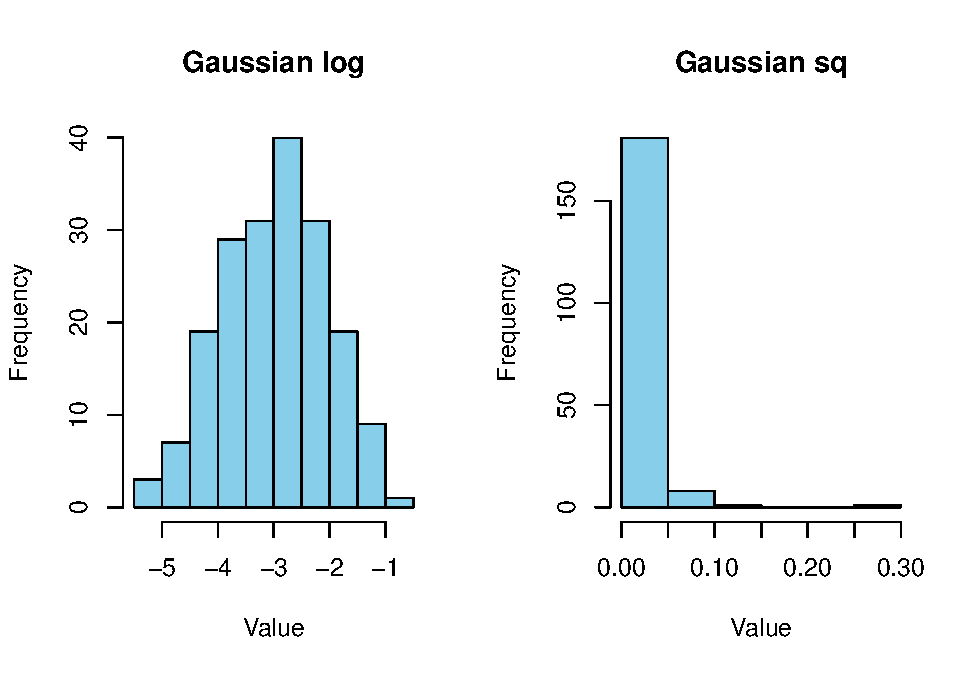
\includegraphics{ts_construction_labor_files/figure-latex/unnamed-chunk-13-1.pdf}

\begin{Shaded}
\begin{Highlighting}[]
\NormalTok{decomposeAltamira }\OtherTok{\textless{}{-}} \FunctionTok{stl}\NormalTok{(ts\_altamira, }\AttributeTok{s.window =} \StringTok{"periodic"}\NormalTok{)}
\FunctionTok{autoplot}\NormalTok{(decomposeAltamira)}
\end{Highlighting}
\end{Shaded}

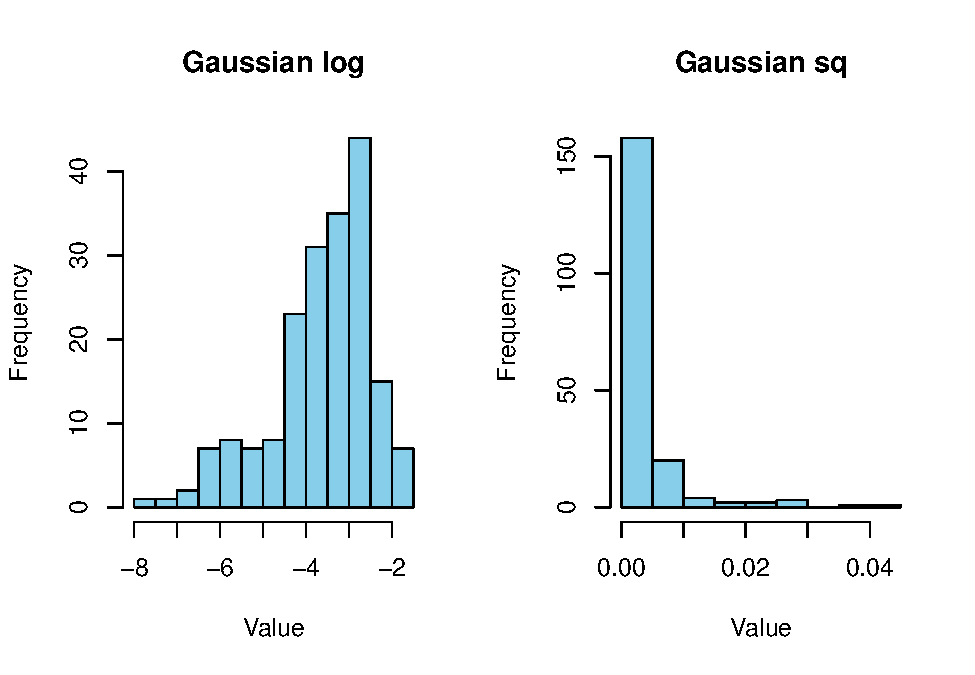
\includegraphics{ts_construction_labor_files/figure-latex/unnamed-chunk-14-1.pdf}

\hypertarget{autocorrelation}{%
\subsection{Autocorrelation}\label{autocorrelation}}

\begin{Shaded}
\begin{Highlighting}[]
\FunctionTok{plot}\NormalTok{(}\FunctionTok{Acf}\NormalTok{(ts\_tucurui), }\AttributeTok{main =} \StringTok{"Autocorrelation Function of Turnover Tucurui"}\NormalTok{)}
\end{Highlighting}
\end{Shaded}

\includegraphics{ts_construction_labor_files/figure-latex/unnamed-chunk-15-1.pdf}
\includegraphics{ts_construction_labor_files/figure-latex/unnamed-chunk-15-2.pdf}

\begin{Shaded}
\begin{Highlighting}[]
\FunctionTok{plot}\NormalTok{(}\FunctionTok{Acf}\NormalTok{(ts\_altamira), }\AttributeTok{main =} \StringTok{"Autocorrelation Function of Turnover Altamira"}\NormalTok{)}
\end{Highlighting}
\end{Shaded}

\includegraphics{ts_construction_labor_files/figure-latex/unnamed-chunk-16-1.pdf}
\includegraphics{ts_construction_labor_files/figure-latex/unnamed-chunk-16-2.pdf}

\hypertarget{correlation-analysis}{%
\subsection{Correlation Analysis}\label{correlation-analysis}}

\begin{Shaded}
\begin{Highlighting}[]
\NormalTok{df\_tucurui }\OtherTok{\textless{}{-}}\NormalTok{ df }\SpecialCharTok{\%\textgreater{}\%}
  \FunctionTok{select}\NormalTok{(}\FunctionTok{matches}\NormalTok{(}\StringTok{"Tucurui"}\NormalTok{))}

\NormalTok{df\_altamira }\OtherTok{\textless{}{-}}\NormalTok{ df }\SpecialCharTok{\%\textgreater{}\%}
  \FunctionTok{select}\NormalTok{(}\FunctionTok{matches}\NormalTok{(}\StringTok{"Altamira"}\NormalTok{))}
\end{Highlighting}
\end{Shaded}

\begin{Shaded}
\begin{Highlighting}[]
\NormalTok{corr\_mat }\OtherTok{\textless{}{-}} \FunctionTok{round}\NormalTok{(}\FunctionTok{cor}\NormalTok{(df\_tucurui), }\DecValTok{2}\NormalTok{)}

\NormalTok{dist }\OtherTok{\textless{}{-}} \FunctionTok{as.dist}\NormalTok{((}\DecValTok{1}\SpecialCharTok{{-}}\NormalTok{corr\_mat)}\SpecialCharTok{/}\DecValTok{2}\NormalTok{)}
 
\CommentTok{\# hierarchical clustering the dist matrix}
\NormalTok{hc }\OtherTok{\textless{}{-}} \FunctionTok{hclust}\NormalTok{(dist)}
\NormalTok{corr\_mat }\OtherTok{\textless{}{-}}\NormalTok{corr\_mat[hc}\SpecialCharTok{$}\NormalTok{order, hc}\SpecialCharTok{$}\NormalTok{order]}
 
\CommentTok{\# reduce the size of correlation matrix}
\NormalTok{melted\_corr\_mat }\OtherTok{\textless{}{-}} \FunctionTok{melt}\NormalTok{(corr\_mat)}
 
\FunctionTok{ggplot}\NormalTok{(}\AttributeTok{data =}\NormalTok{ melted\_corr\_mat, }\FunctionTok{aes}\NormalTok{(}\AttributeTok{x =}\NormalTok{ Var1, }\AttributeTok{y =}\NormalTok{ Var2, }\AttributeTok{fill =}\NormalTok{ value)) }\SpecialCharTok{+} 
  \FunctionTok{geom\_tile}\NormalTok{() }\SpecialCharTok{+}
  \FunctionTok{geom\_text}\NormalTok{(}\FunctionTok{aes}\NormalTok{(Var2, Var1, }\AttributeTok{label =}\NormalTok{ value), }\AttributeTok{color =} \StringTok{"black"}\NormalTok{, }\AttributeTok{size =} \DecValTok{4}\NormalTok{) }\SpecialCharTok{+}
  \FunctionTok{theme\_minimal}\NormalTok{() }\SpecialCharTok{+}
  \FunctionTok{theme}\NormalTok{(}\AttributeTok{axis.text.x =} \FunctionTok{element\_text}\NormalTok{(}\AttributeTok{angle =} \DecValTok{90}\NormalTok{, }\AttributeTok{vjust =} \FloatTok{0.5}\NormalTok{, }\AttributeTok{hjust =} \DecValTok{1}\NormalTok{),}
        \CommentTok{\#plot.margin = unit(c(0.02, 0.02, 0.02, 0.02), "mm")}
\NormalTok{        )}
\end{Highlighting}
\end{Shaded}

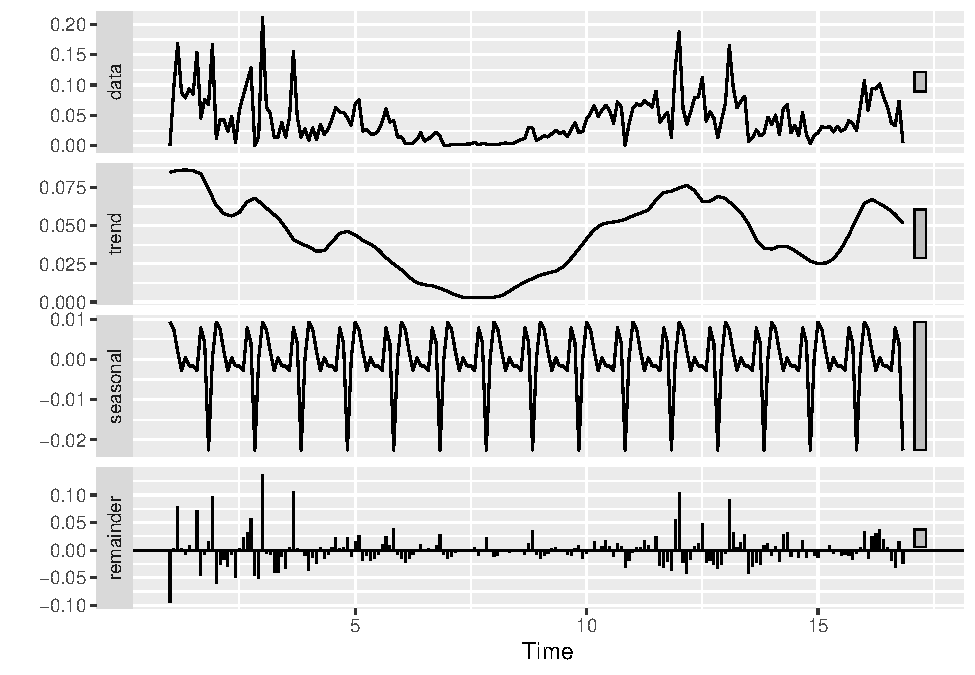
\includegraphics{ts_construction_labor_files/figure-latex/unnamed-chunk-18-1.pdf}

\begin{Shaded}
\begin{Highlighting}[]
\FunctionTok{ggsave}\NormalTok{(}\StringTok{"corr\_tucurui.png"}\NormalTok{, }\AttributeTok{plot =}\NormalTok{ gg, }\AttributeTok{width =} \DecValTok{10}\NormalTok{, }\AttributeTok{height =} \DecValTok{8}\NormalTok{, }\AttributeTok{units =} \StringTok{"in"}\NormalTok{, }\AttributeTok{dpi =} \DecValTok{300}\NormalTok{)}
\end{Highlighting}
\end{Shaded}

\begin{Shaded}
\begin{Highlighting}[]
\NormalTok{corr\_mat }\OtherTok{\textless{}{-}} \FunctionTok{round}\NormalTok{(}\FunctionTok{cor}\NormalTok{(df\_altamira), }\DecValTok{2}\NormalTok{)}

\NormalTok{dist }\OtherTok{\textless{}{-}} \FunctionTok{as.dist}\NormalTok{((}\DecValTok{1}\SpecialCharTok{{-}}\NormalTok{corr\_mat)}\SpecialCharTok{/}\DecValTok{2}\NormalTok{)}
 
\CommentTok{\# hierarchical clustering the dist matrix}
\NormalTok{hc }\OtherTok{\textless{}{-}} \FunctionTok{hclust}\NormalTok{(dist)}
\NormalTok{corr\_mat }\OtherTok{\textless{}{-}}\NormalTok{corr\_mat[hc}\SpecialCharTok{$}\NormalTok{order, hc}\SpecialCharTok{$}\NormalTok{order]}
 
\CommentTok{\# reduce the size of correlation matrix}
\NormalTok{melted\_corr\_mat }\OtherTok{\textless{}{-}} \FunctionTok{melt}\NormalTok{(corr\_mat)}
 
\FunctionTok{ggplot}\NormalTok{(}\AttributeTok{data =}\NormalTok{ melted\_corr\_mat, }\FunctionTok{aes}\NormalTok{(}\AttributeTok{x =}\NormalTok{ Var1, }\AttributeTok{y =}\NormalTok{ Var2, }\AttributeTok{fill =}\NormalTok{ value)) }\SpecialCharTok{+} 
  \FunctionTok{geom\_tile}\NormalTok{() }\SpecialCharTok{+}
  \FunctionTok{geom\_text}\NormalTok{(}\FunctionTok{aes}\NormalTok{(Var2, Var1, }\AttributeTok{label =}\NormalTok{ value), }\AttributeTok{color =} \StringTok{"black"}\NormalTok{, }\AttributeTok{size =} \DecValTok{4}\NormalTok{) }\SpecialCharTok{+}
  \FunctionTok{theme}\NormalTok{(}\AttributeTok{axis.text.x =} \FunctionTok{element\_text}\NormalTok{(}\AttributeTok{angle =} \DecValTok{90}\NormalTok{, }\AttributeTok{vjust =} \FloatTok{0.5}\NormalTok{, }\AttributeTok{hjust=}\DecValTok{1}\NormalTok{)) }
\end{Highlighting}
\end{Shaded}

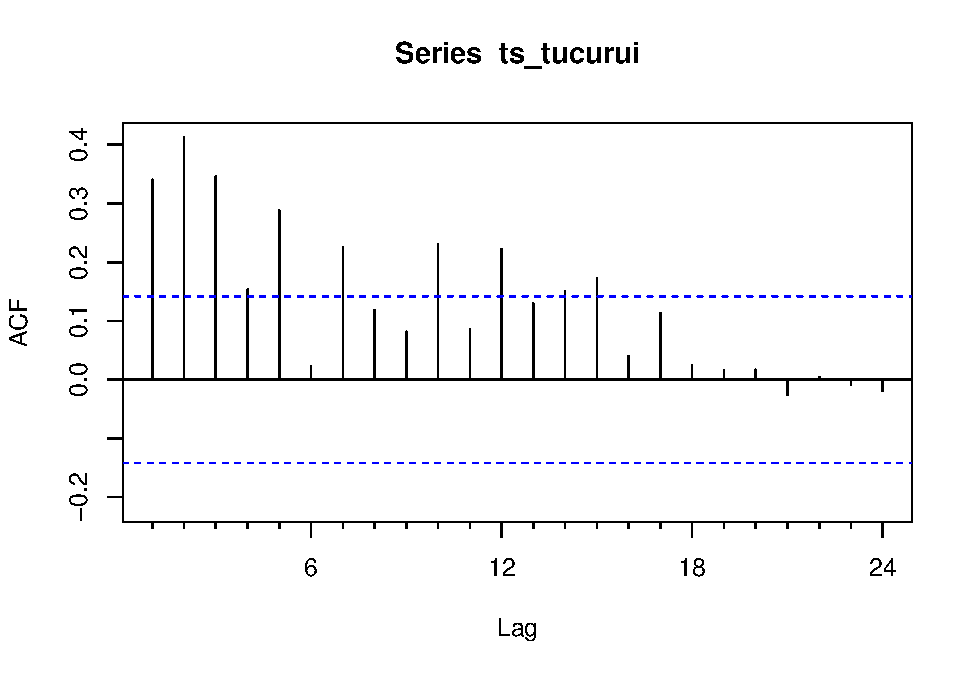
\includegraphics{ts_construction_labor_files/figure-latex/unnamed-chunk-19-1.pdf}

\end{document}
